% =====================================================================
%  Northeastern Economics -- working paper template (pdflatex)
% =====================================================================
\documentclass[12pt]{article}
\usepackage[utf8]{inputenc}
\usepackage[margin=1in]{geometry}
\usepackage{mathpazo}
\usepackage{amsmath,amssymb,amsthm}
\usepackage{setspace}\onehalfspacing
\usepackage{booktabs,threeparttable}
\usepackage{graphicx}
\usepackage{pgfplots}\pgfplotsset{compat=1.16}
\usepackage[authoryear,round]{natbib}
\usepackage[colorlinks=true,linkcolor=blue!60!black,citecolor=blue!60!black,urlcolor=blue!60!black]{hyperref}

\newtheorem{proposition}{Proposition}

\title{Title of Your Paper\thanks{Acknowledgements. Contact: \texttt{your.name@northeastern.edu}.}}
\author{Your Name\\ \small Department of Economics, Northeastern University}
\date{\today}

\begin{document}
\maketitle

\begin{abstract}
\noindent One paragraph: question, setting and data, method, main result, and why it matters.
\medskip

\noindent\textbf{JEL codes:} L00, D00. \quad \textbf{Keywords:} keyword one, keyword two.
\end{abstract}

\section{Introduction}
State the question and the answer early. Position the paper relative to prior work
\citep{placeholderA} and say what is new \citep[see also][]{placeholderB}.

\section{Model}
A consumer chooses consumption $q_t$ and purchases $x_t$ to solve
\begin{equation}
\max_{\{x_t,q_t\}} \sum_{t=1}^{T}\bigl[u(q_t)+n_t\bigr]
\quad\text{s.t.}\quad \sum_{t=1}^{T}\bigl(p_t x_t+n_t\bigr)\le T y .
\label{eq:problem}
\end{equation}
\begin{proposition}
State a result implied by \eqref{eq:problem}.
\end{proposition}

\section{Data and empirical strategy}
Describe the data source and estimating equation:
\begin{equation}
\log q_{jmt}=\alpha_{mj}-\beta\,p_{jmt}+X_{jmt}'\gamma+\varepsilon_{jmt}.
\end{equation}

\section{Results}
Table~\ref{tab:main} reports estimates and Figure~\ref{fig:demand} plots the fitted relationship.

\begin{table}[ht]\centering
\begin{threeparttable}
\caption{Main estimates}\label{tab:main}
\begin{tabular}{lccc}
\toprule
 & (1) OLS & (2) IV & (3) IV + FE\\
\midrule
Price & $-0.00$ & $-0.00$ & $-0.00$\\
      & (0.00) & (0.00) & (0.00)\\
\midrule
Fixed effects & No & No & Yes\\
Observations  & 0 & 0 & 0\\
\bottomrule
\end{tabular}
\begin{tablenotes}\footnotesize
\item Notes: Placeholder values. Standard errors in parentheses.
\end{tablenotes}
\end{threeparttable}
\end{table}

\begin{figure}[ht]\centering
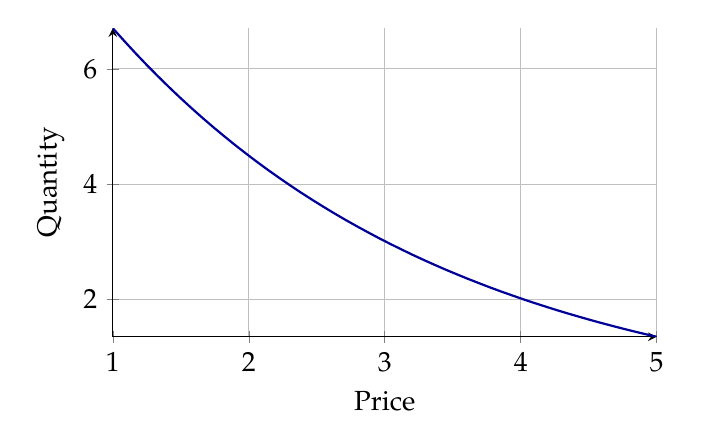
\begin{tikzpicture}
\begin{axis}[width=0.7\linewidth,height=5.5cm,xlabel={Price},ylabel={Quantity},axis lines=left,grid=major]
\addplot[thick,blue!60!black,domain=1:5,samples=50]{10*exp(-0.4*x)};
\end{axis}
\end{tikzpicture}
\caption{Illustrative demand curve (placeholder).}\label{fig:demand}
\end{figure}

\section{Conclusion}
Summarize findings, limitations, and next steps.

\begin{thebibliography}{9}
\bibitem[Author(Year)]{placeholderA} Author, A. (Year). Title of a related paper. \textit{Journal Name}.
\bibitem[Author and Coauthor(Year)]{placeholderB} Author, B. and Coauthor, C. (Year). Title of another related paper. \textit{Journal Name}.
\end{thebibliography}

\end{document}
